\documentclass[10pt, conference]{IEEEtran}
\hyphenation{op-tical net-works semi-conduc-tor}
\usepackage{graphicx}
\usepackage{fancyhdr}
\usepackage{url}
\usepackage{amsmath}
\usepackage{listings}
\usepackage{algorithm}
\usepackage{algorithmic}
\usepackage{lipsum}
\usepackage[table,xcdraw]{xcolor}
\usepackage{bookmark}
\usepackage[normalem]{ulem}
\def\code#1{\texttt{#1}}
\useunder{\uline}{\ul}{}
\usepackage{setspace}
\doublespacing

\pagestyle{fancy}
\fancyhf{}
\lhead{\textsc{ELEN4020}}
\rhead{\textsc{Group 9: Project 2018}}
\rfoot{Page \thepage\ }


\begin{document}
\begin{titlepage}
\newcommand{\HRule}{\rule{\linewidth}{0.5mm}} % Defines a new command for the horizontal lines, change thickness here

\center % Center everything on the page
 
%----------------------------------------------------------------------------------------
%	HEADING SECTIONS
%----------------------------------------------------------------------------------------

\textsc{\LARGE University of Witwatersrand}\\[1.5cm] % Name of your university/college
%----------------------------------------------------------------------------------------
%	LOGO SECTION
%----------------------------------------------------------------------------------------


\includegraphics[scale=0.25]{Wits.png}% Include a department/university logo - this will require the graphicx package
 
 
%----------------------------------------------------------------------------------------
\textsc{\Large ELEN4020}\\[0.5cm] % Major heading such as course name
\textsc{\large Data Intensive Computing in Data Science}\\[0.5cm] % Minor heading such as course title



%----------------------------------------------------------------------------------------
%	TITLE SECTION
%----------------------------------------------------------------------------------------

\HRule \\[0.4cm]
{ \huge \bfseries Group 9: Project 2018}\\[0.4cm] % Title of your document
\HRule \\[1.5cm]
 
%----------------------------------------------------------------------------------------
%	AUTHOR SECTION
%----------------------------------------------------------------------------------------
\singlespacing
\begin{minipage}{0.4\textwidth}
\begin{flushleft} \large
	\emph{Authors:}\\
	\textsc{Kishan Narotam - 717 931\\Jesal Chana - 603 177} 
\end{flushleft}
\end{minipage}
~
\begin{minipage}{0.4\textwidth}
\begin{flushright} \large
	\emph{Authors:} \\
	\textsc{Syed Hussain - 600 524\\Yusuf Ally - 604 973} 
\end{flushright}
\end{minipage}\\[1cm]

%----------------------------------------------------------------------------------------
%	DATE SECTION
%----------------------------------------------------------------------------------------

{\large 15\textsuperscript{th} May 2018}\\[1cm] % Date, change the \today to a set date if you want to be precise

%-------------------------------------------------------------------------------------

%----------------------------------------------------------------------------------------
%	ABSTRACT SECTION
%----------------------------------------------------------------------------------------
 

\begin{abstract}
The design and implementation of two parallel equi-join algorithms (MPI and OpenMP) have been presented. Two relational tables, $F_1$ and $F_2$ of a user-chosen size can be generated using a C++ program created called \code{tableGenerator.cpp} and these tables are written to external files, \code{F\textsubscript{1}.txt} and \code{F\textsubscript{2}.txt} respectively. Table $F_1$ contains two columns, a key (integer) and a randomly generated string (5 uppercase letters), while table $F_2$ contains two columns, a key (integer) and a randomly generated string (8 lowercase letters), and said tables must be joined on the common attribute, being the key and stored in table $F_3$ stored in \code{F\textsubscript{3}.txt}. High-level algorithms are given for the table generator, MPI algorithm and OpenMP algorithm with various strengths and limitations presented. The experimental and testing environment of the built cluster and a benchmark device has been expanded on and results of various table sizes and various threads used have been tabulated and graphically presented in order to display the scalability and speed of the algorithms. Due to various time constraints, the full implementation of the MPI algorithm was not possible due to send and receive requests that was being blocked by the code and as a result of this, no testing could be done for the MPI algorithm. However, the MPI algorithm should be faster on the cluster than the OpenMP algorithm.

All source code and documentation can be found on the GitHub repository link: \url{https://github.com/KNarotam/ELEN4020---Data-Intensive-Computing-In-Data-Science}
\end{abstract}
\doublespacing
%----------------------------------------------------------------------------------------

\vfill % Fill the rest of the page with whitespace

\end{titlepage}
%----------------------------------------------------------------------------------------

%----------------------------------------------------------------------------------------
%	MAIN BODY OF REPORT
%----------------------------------------------------------------------------------------

\section{Introduction}
\label{sec: Introdution}
Large corporations such as \emph{Facebook}, \emph{Google}, \emph{Microsoft} and \emph{IBM} have constantly increasing databases. The maintenance of these databases require dedicated time and plentiful resources. As new entries are constantly added to the database, it continues to get larger. One method of maintaining the database would be to delete unwanted, unnecessary data~\cite{IBM Maintaining}.

In most cases, data is spread across various databases each storing specific types of data. For example, in an insurance company, one database table could be utilized for storing the records of all members that have life insurance, while another database table stores the records of all members that have medical insurance. In a situation like this, combining the two tables would aid the company in accessing all the relevant information stored for a specific member.

In the report that follows two algorithms are implemented using equi-join of two very large tables on their common join attributes. The first algorithm utilizes MPI (Message Passing Interface), while the second utilizes OpenMP. The algorithms are then tested on a cluster, which is explained, as well as a single separate computer that will be used as a benchmark for the algorithms, and the results presented.

\section{Background}
\label{sec: Background}

\subsection{Requirements}
\label{sec: Requirements}
The requirement of this project is develop two algorithms that implement a parallel equi-join of two very large tables on the common join attribute. The two tables are stored and maintained in two files, \code{F\textsubscript{1}.txt} and \code{F\textsubscript{2}.txt}. Given that table $F_1$ has attributes ($A,B$) and table $F_2$ with attributes ($A,C$), these tables must be joined on attribute $A$ to produce relational table $F_3$ with attributes ($A,B,C$) which must then be written and stored to file \code{F\textsubscript{3}.txt}.

One of the join algorithms utilized must use MPI. A straight forward MPI distributed programming model with one of of the other programming models, in this case, OpenMP, will be utilized in this project. The purpose of having two different programming models is to allow for comparative performance analysis.

\subsection{Constraints}
\label{sec: Constraints}
The join algorithms used must be equi-join and not any other type of join algorithms such as left join, inner join, etc. Additionally, one of the algorithms must use MPI and all testing must be done on the built cluster.

\subsection{Success Criteria}
\label{sec: Success Criteria}
The project and subsequently the algorithms can be considered a success if the requirements mentioned in Section~\ref{sec: Requirements} are met. Consequently, the joined tables must be tested on the cluster and the output files must be written to the file $F_3$.

\section{Algorithms}
\label{sec: Algorithms}

\subsection{Table Generator}
\label{section: Table Generator}
The two relational tables, $F_1$ and $F_2$, that will be joined are generated using a user-created C++ program named \code{tableGenerator.cpp}. The function of this program generates the two tables with the user choosing the size of the table. In table $F_1$, stored in the external file \code{F\textsubscript{1}.txt}, the first column is the key (the joining attribute), and the second column is a randomly generated string of five upper-case letters. Subsequently, in table $F_2$, stored in the external file \code{F\textsubscript{2}.txt}, the first column is the key (joining attribute) and the second column is a randomly generated string of eight lower-case letters.

Within this file, four global variables are declared, and two functions that return random letters. The \code{main} function of the class calls these methods and writes the tables to the respective text files. Algorithm~\ref{alg: tableGenerator} shows a high level algorithm of the \code{tableGenerator.cpp} file.

\begin{algorithm}[h!]
\caption{High level algorithm of the \code{tableGenerator.cpp} class}
\label{alg: tableGenerator}
\begin{algorithmic}
\STATE \textbf{Input:} $tableSize$
\STATE
\STATE create the upper-case letters \code{char} array 
\STATE create the lower-case letters \code{char} array
\STATE calculate size of arrays
\STATE
\STATE \textbf{Function}\{\code{getUpperChar}\}
\STATE \qquad \textbf{return} random \code{char} from upper-case array
\STATE \textbf{end Function}
\STATE \textbf{Function}\{\code{getLowerChar}\}
\STATE \qquad \textbf{return} random \code{char} from lower-case array
\STATE \textbf{end Function}
\STATE
\STATE create the two text files $F_1.txt$ and $F_2.txt$
\STATE define string length for table 1 to be 5
\STATE define string length for table 2 to be 8
\STATE User input
\FOR{\code{i = 0} till \code{tableSize}}
	\STATE Generate random string for table 1 and table 2
	\STATE Write key and string values to $F_1.txt$ and $F_2.txt$
\ENDFOR
\RETURN 0
\end{algorithmic}
\end{algorithm}

The user is able to define the size of the table that will be generated as this value will change for testing purposes.

\subsection{MPI Algorithm}
\label{sec: MPI Algorithm}
The main algorithm uses the MPI (Message Passing Interface Standard) which addresses the message-passing parallel programming model. As opposed to being an IEEE standard, MPI has become somewhat of an industry standard~\cite{MPI}. The master node reads in a single line of table $F_1$ and broadcasts that key to all the other nodes in the cluster using \code{MPI\_Bcast()}. A second broadcast is done to send the value of table $F_1$ that corresponds to that key. This distributes the current key to every node to search for any equal keys in table $F_1$. Since all the slave nodes have access to the home directory each node will read a range of table $F_2$ corresponding to its rank using Equations~\ref{eqn: MPI1},~\ref{eqn: MPI2} and~\ref{eqn: MPI3}.

Then each slave calculates its search range by calculating the required lower and upper bounds by using its specific rank and Equation~\ref{eqn: MPI1}. The upper bound limit is compared to a global variable \code{numberOfEntries}. If the calculated upper limit is greater than \code{numberOfEntries} then the upper limit is set to equal \code{numberOfEntries} to prevent indexing errors. Once the upper and lower bounds have been calculated and the current key has been distributed using the broadcast each slave node can begin to iterate through the portions of the table that corresponds to its set search range and will compare the keys on every iteration to the distributed key from table $F_1$. On a successful equality of keys the slave node will send the master the index at which $F_2$ has the same as the key given from table $F_1$. The master then gets the key, the corresponding value from table $F_1$, and the corresponding value from table $F_2$. Then it joins the values from tables $F_1$ and $F_2$ and writes the result to a file in the master node’s home directory called \code{F\textsubscript{3}.txt}.

Unfortunately, due to time constraints the full implementation of this algorithm was not possible and during send and receive requests the code was blocking. To counteract this a local memory version of the algorithm was implemented which would not be able to run on the distributed cluster, however, with changes to the \code{MPI\_send} and \code{MPI\_recieve} commands to handle it on a distributed system.

\begin{equation}
\label{eqn: MPI1}
\begin{split}
Chunk\ size = \frac{Number\ of\ Entries}{Number\ of\ Nodes}
\end{split}
\end{equation}
where: $Chunk\ size$ defines the number of values that each node will iterate through; $Number\ of\ entries$ is the total number of entries for table $F_2$; and $Number\ of\ nodes$ is the number of nodes that will carry out searches.

\begin{equation}
\label{eqn: MPI2}
\begin{split}
Lower\ limit = Rank \times Chunk\ size
\end{split}
\end{equation}
where: $Lower\ limit$ is the start of the search range for this node; $Rank$ is the unique rank given to the nodes that are searching; and $Chunk\ size$ defines the number of values that each node will iterate through.

\begin{equation}
\label{eqn: MPI3}
\begin{split}
Upper\ limit = \left([Rank+1]\times Chunk\ size\right)-1
\end{split}
\end{equation}
where: $Upper\ limit$ defines the final element in the nodes search range; $Rank$ is the unique rank given to the nodes that are searching; and $Chunk\ size$ defines the number of values that each node will iterate through.

\subsubsection{Strengths}
\label{sec: Strengths}
\begin{itemize}
\item The algorithm makes use of the parallel structure of the cluster efficiently, by delegating search ranges to each slave node. This allows $F_2$ to be read up to $N$ times faster, where $N$ is the number of slaves, this excludes delegation and send times by the master.
\item The solution is scalable as the block size of $F_2$ is dependent on the number of available nodes. As more nodes are added, the master node is able to delegate blocks to maximize the number of nodes for a particular table size.
\end{itemize}

\subsubsection{Limitations}
\label{sec: Limitations}
\begin{itemize}
\item Each slave has to read from the same master data and so this can cause a bottleneck if the communication bandwidth is insufficient. 
\item The number of elements needs to be divisible by the number of process, if not then the final process will receive less search elements to read through than the other slave nodes.
\item Since the data is read by the master node into its local storage it means that the algorithm requires enough storage space to hold the table file in its original form as well as in the vector in memory.
\item The size and elements of the Tables are required before accurate distribution of data elements and search ranges.
\end{itemize}

\subsubsection{Improvements}
\label{sec: Improvements}
\begin{itemize}
\item Using scatter and a dynamic file read can improve performance issues relating to storage size and bandwidth problems. \code{MPI\_Scatter()} partitions the given data  By using a dynamic file read we can reduce the total size of the table in memory by removing entries that have been sent to a slave node via scatter. 
\item Using \code{struct}s to broadcast information and to do storage and joins will lead to a more robust and flexible solution which can handle different types of values and data types.
\end{itemize}

\subsection{OpenMP Algorithm}
\label{sec: OpenMP Algorithm}
The second algorithm uses OpenMP with the nested \code{for} join. OpenMP (Open Multi-Processing) is an an application program interface (API) that is used specifically for parallel programming. It is regarded as a much higher level API, and portable allowing OpenMP to be utilized in a variety of languages such as C, C++ and Fortran. It is more easily scaled than PThreads, as it has the ability to divide the work across multiple threads with ease~\cite{OpenMP}.

The algorithm allocates a master thread and slave threads, the total of which equal the number of processing nodes available. Table $F_1$ and Table $F_2$ are generated using the \code{tableGenerator.cpp} and are stored in the shared memory of the cluster, i.e. these files are accessed through all of the nodes. The tables are loaded from the shared memory via the master thread and is read in line by line.

Once the data is read in, an OpenMP lock is created. The purpose of the lock is to guarantee that the next set of instructions can only be performed one process at a time, i.e. it prevents different threads from simultaneously changing the same data~\cite{OpenMP}. A set of global variables are then shared between the slave threads. These variables are: a lock variable to allow a thread to lock a process, Table $F_2$, Table $F_3$, the size of Table $F_1$ and the size of Table $F_2$.

The join algorithm used with OpenMP is similar to that of the brute-force nested loop join with no partitioning stage. The nested \code{for} loop is used to iterate 	through the chunk given to each thread. A key value pair is stored in a temporary variable in the first \code{for} loop and is passed to a second \code{for} where the key of the temporary variable is compared to all the values in Table $F_2$. Using an \code{if} statement, the keys are tested for equality, and when the keys match, an entry is added Table $F_3$ with the corresponding key and string values from Table $F_1$ and Table $F_2$. This process is done on a locked thread. Algorithm~\ref{alg: OpenMP} shows a high level algorithm of the \code{openMP.cpp} file.

\begin{algorithm}[h!]
\caption{High level algorithm of the \code{openMP.cpp} class}
\label{alg: OpenMP}
\begin{algorithmic}
\STATE \textbf{Input:} $NUM\_THREADS$
\STATE
\STATE read $F_1.txt$ and store in array of $key$-$value$ pairs
\STATE read $F_2.txt$ and store in array of $key$-$value$ pairs
\STATE ask user to set $NUM\_THREADS$
\STATE set number of threads
\STATE initialize \code{omp\_lock}
\STATE initialize threads with shared variables
\STATE int \code{count} $\leftarrow 0$
\STATE 
\FOR{\code{i = 0} till size of $F_1.txt$}
	\STATE \code{tempKeyA} $\leftarrow$ \code{keyA[i]}
	\FOR{\code{j = 0} till size of $F_2.txt$}
		\STATE \code{tempKeyB} $\leftarrow$ \code{keyB[j]}
		\IF{\code{tempKeyA} = \code{tempKeyB}}
			\STATE set \code{omp\_lock}
			\STATE \code{C[i]} $\leftarrow$ \code{A[i]+ " " + B[i]}
			\STATE \code{count}++
			\STATE unset \code{omp\_lock}
		\ENDIF
	\ENDFOR
\ENDFOR
\STATE write joined table to file $F_3.txt$
\RETURN 0
\end{algorithmic}
\end{algorithm}

\section{Experimental Environment}
\label{sec: Experimental Environment}

\subsection{Cluster}
\label{sec: Cluster}
\begin{figure*}[h!]
\renewcommand{\thefigure}{\arabic{figure}}
\centering
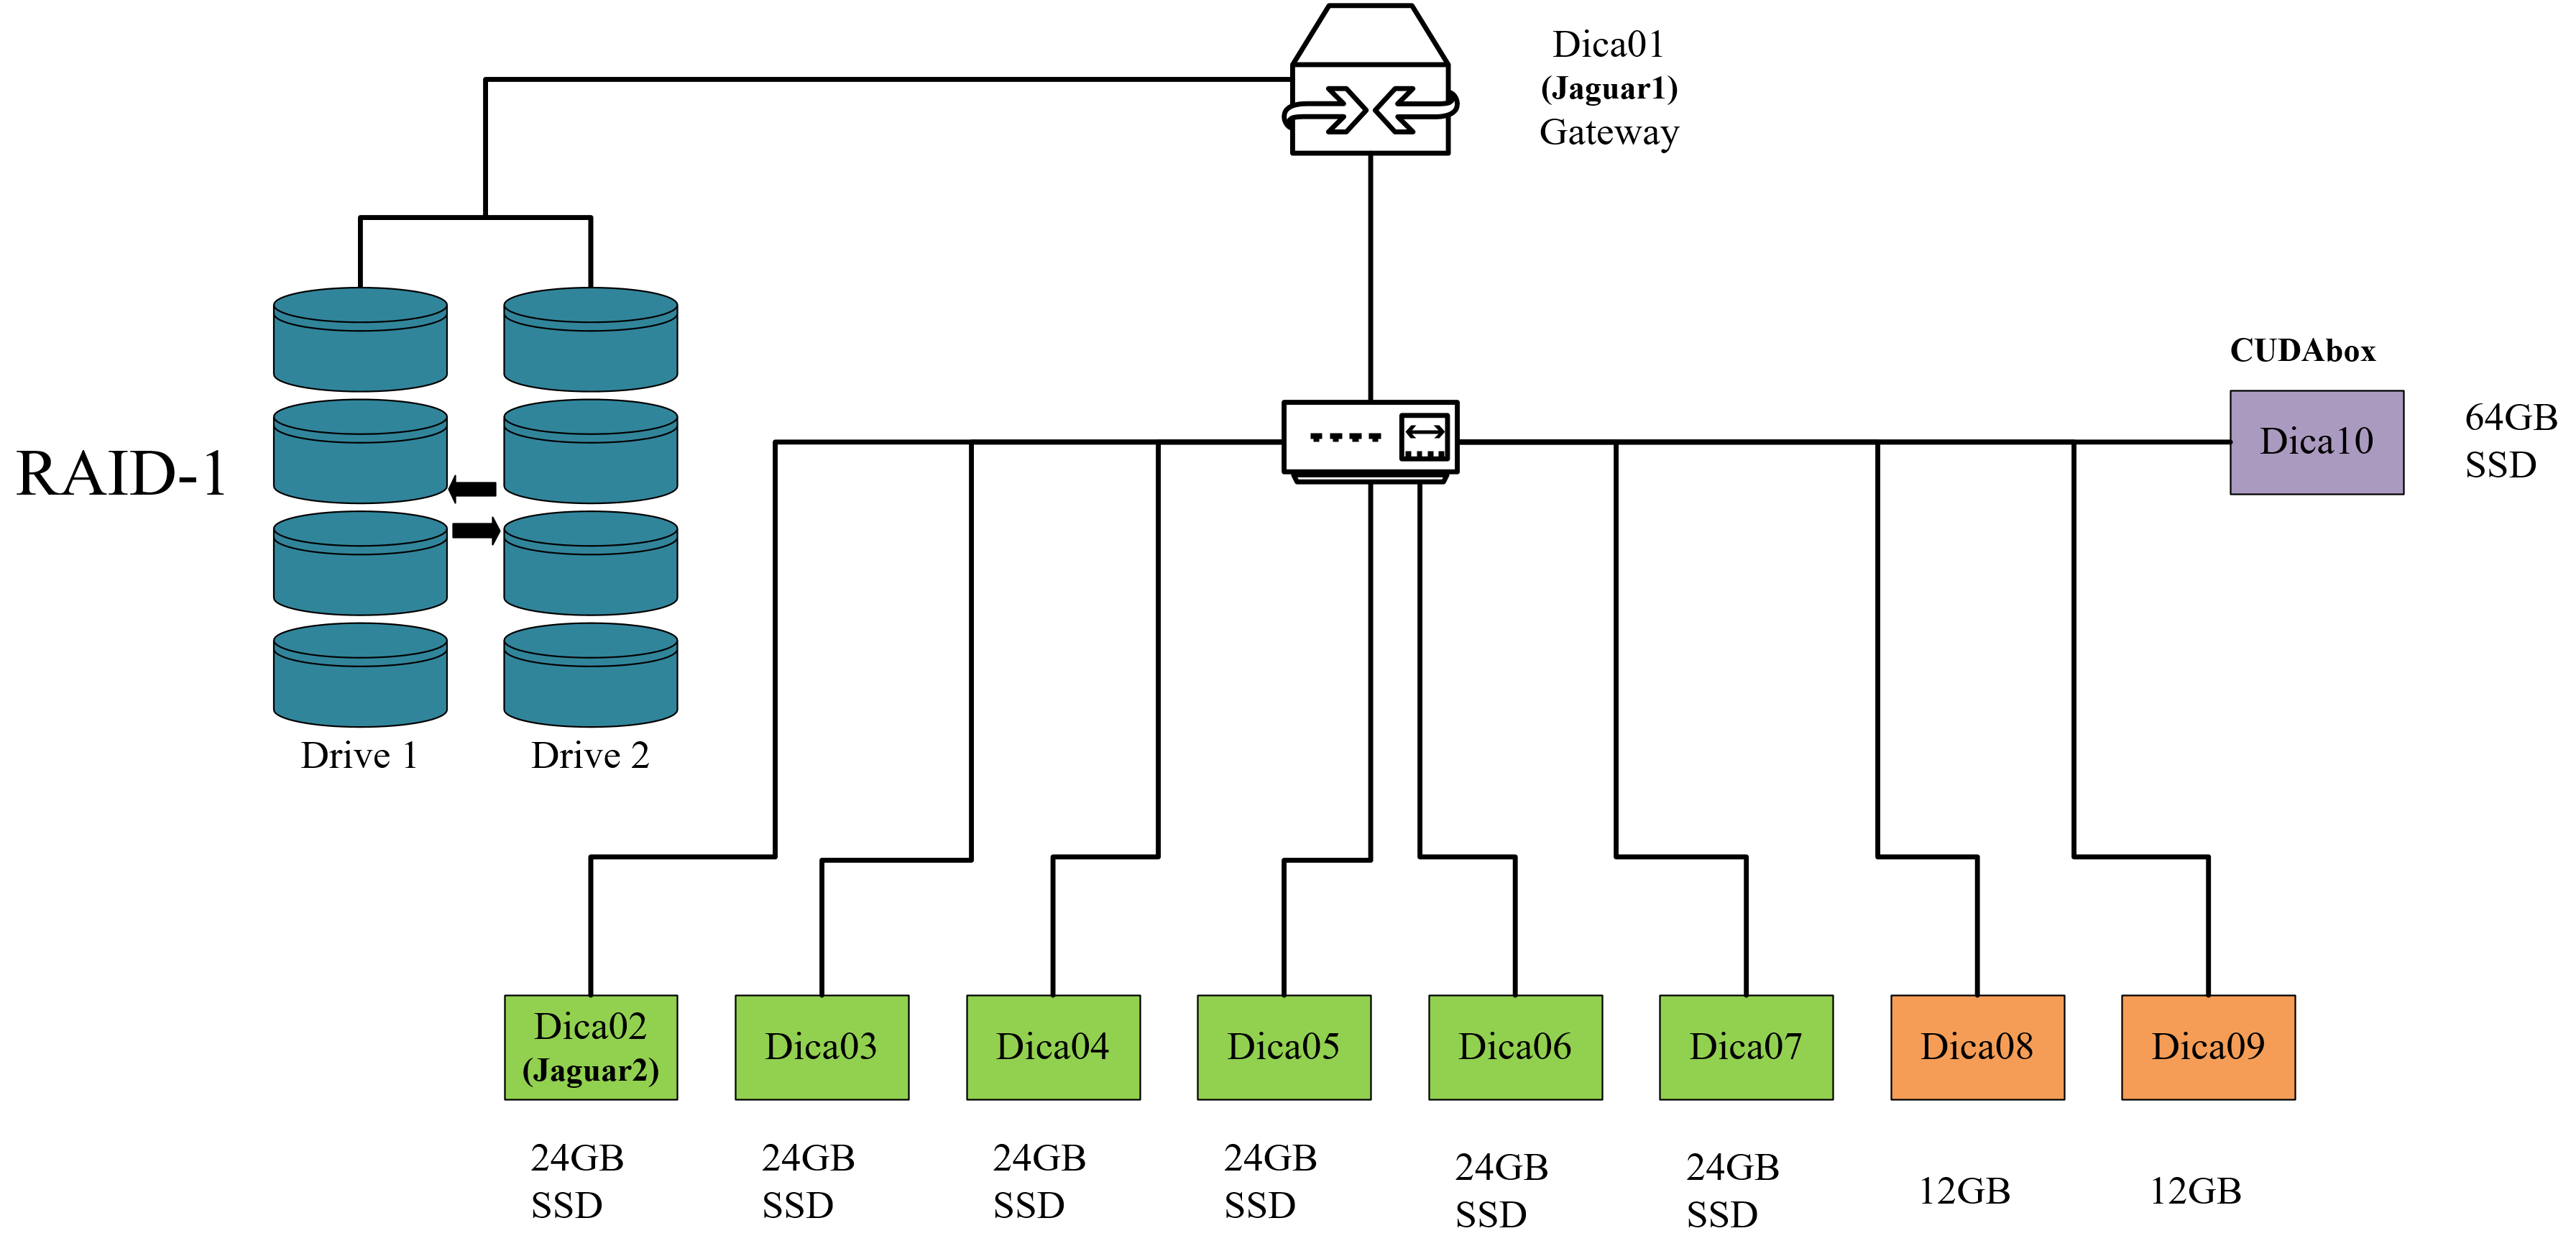
\includegraphics[scale=0.3]{Cluster.png}
\caption{Diagram showing the basis of the cluster, the nodes' memory and type of hard disk drives}
\label{fig: Cluster}
\end{figure*}

A computer cluster was created for the testing purposes of the project. A computer cluster is defined as a single logical unit whereby multiple computers are linked together through a LAN. These networked computers now act as a single machine with more power, increasing processing speed, the storage capacity, improving the data integrity and reliability. The advantage of working within a cluster allows for large data processing, an increase in speed of data processing and provides users a high availability of resources~\cite{Cluster definition}. Figure~\ref{fig: Cluster} shows the basis of the cluster design and architecture.

The cluster begins from RAID-1, or disk mirroring. A redundant array of independent disks (RAID) is defined as a method of grouping individual physical drives together in order to form a bigger drive called a RAID set. There are various types of RAID sets, which are defined by level numbers, whereby RAID-0, RAID-1 and RAID-5 are the most common. In this cluster, a RAID-1 set is used, which is regarded as the most reliable. It allows for no data to be lost across the hard disk drives and synchronously mirrors the data from each hard disk drive to an exact duplicate~\cite{RAID}.

In order to access the cluster, the user must first Secure Shell (SSH) via a terminal such as \emph{PuTTY}. The user will then log into \emph{Jaguar1} or \emph{Dica01}, and using a \code{machine} file, the user will be able to use the nodes \emph{Dica02} till \emph{Dica09}. The user can determine the number of nodes that will be utilized in processing the different algorithms.

\subsection{ASUS}
\label{sec: ASUS}
An ASUS N550JV high performance laptop was used as a ``benchmark" for the OpenMP testing. The machine has an \emph{Intel(R) Core(TM) i7-4700HQ CPU} with $12GB$ of RAM installed with a 64-bit operating system installed. The operating system installed is \emph{Ubuntu 16.04 LTS}.

\section{Results}
\label{sec: Results}

\subsection{MPI Results}
\label{sec: MPI Results}
Due to time constraints, and an unforeseen error on the cluster, thorough testing of the MPI algorithm could not be done. As the benchmark computer used could not simulate 2 nodes (processes) due to the error of the send and receive requests were being blocked by the code itself. Theoretically, the MPI algorithm, if programmed correctly should yield faster times.

\subsection{OpenMP Results}
\label{sec: OpenMP Results}
\begin{table*}[h!]
\centering
\caption{Table showing the time taken (in seconds) to perform the join algorithm on the \emph{ASUS} laptop and on \emph{Dica02} on the Cluster}
\label{tbl: OpenMP}
\begin{tabular}{|l|l|l|l|l|l|l|l|l|}
\hline
\multicolumn{3}{|c|}{\cellcolor[HTML]{C0C0C0}{\ul \textbf{Threads = 0}}} & \multicolumn{3}{c|}{\cellcolor[HTML]{C0C0C0}{\ul \textbf{Threads = 4}}} & \multicolumn{3}{c|}{\cellcolor[HTML]{C0C0C0}{\ul \textbf{Threads = 8}}} \\ \hline
\multicolumn{1}{|c|}{{\ul \textbf{Table Size}}} & \multicolumn{1}{c|}{{\ul \textbf{ASUS}}} & \multicolumn{1}{c|}{{\ul \textbf{Cluster}}} & \multicolumn{1}{c|}{{\ul \textbf{Table Size}}} & \multicolumn{1}{c|}{{\ul \textbf{ASUS}}} & \multicolumn{1}{c|}{{\ul \textbf{Cluster}}} & {\ul \textbf{Table Size}} & {\ul \textbf{ASUS}} & {\ul \textbf{Cluster}} \\ \hline
\textbf{10} & 0.000505 & 0.000427 & \textbf{10} & 0.000691 & 0.00848 & \textbf{10} & 0.020215 & 0.029212 \\ \hline
\textbf{100} & 0.000451 & 0.000653 & \textbf{100} & 0.001585 & 0.008773 & \textbf{100} & 0.060356 & 0.028056 \\ \hline
\textbf{500} & 0.008197 & 0.00311 & \textbf{500} & 0.009749 & 0.014723 & \textbf{500} & 0.055863 & 0.036726 \\ \hline
\textbf{1000} & 0.019902 & 0.012039 & \textbf{1000} & 0.048367 & 0.028535 & \textbf{1000} & 0.052915 & 0.050996 \\ \hline
\textbf{2000} & 0.035553 & 0.042524 & \textbf{2000} & 0.077996 & 0.073102 & \textbf{2000} & 0.125781 & 0.106062 \\ \hline
\textbf{5000} & 0.161803 & 0.249228 & \textbf{5000} & 0.232968 & 0.375876 & \textbf{5000} & 0.324462 & 0.435307 \\ \hline
\textbf{10000} & 1.20043 & 0.977631 & \textbf{10000} & 0.844848 & 1.4016 & \textbf{10000} & 1.0934 & 1.68316 \\ \hline
\textbf{50000} & 15.6016 & 24.1215 & \textbf{50000} & 16.1613 & 32.6204 & \textbf{50000} & 27.6152 & 45.6045 \\ \hline
\textbf{100000} & 63.3261 & 97.2487 & \textbf{100000} & 98.6917 & 122.211 & \textbf{100000} & 136.779 & 186.858 \\ \hline
\multicolumn{3}{|c|}{\cellcolor[HTML]{C0C0C0}{\ul \textbf{Threads = 16}}} & \multicolumn{3}{c|}{\cellcolor[HTML]{C0C0C0}{\ul \textbf{Threads = 64}}} & \multicolumn{3}{c|}{\cellcolor[HTML]{C0C0C0}{\ul \textbf{Threads = 128}}} \\ \hline
\multicolumn{1}{|c|}{{\ul \textbf{Table Size}}} & \multicolumn{1}{c|}{{\ul \textbf{ASUS}}} & \multicolumn{1}{c|}{{\ul \textbf{Cluster}}} & \multicolumn{1}{c|}{{\ul \textbf{Table Size}}} & \multicolumn{1}{c|}{{\ul \textbf{ASUS}}} & \multicolumn{1}{c|}{{\ul \textbf{Cluster}}} & {\ul \textbf{Table Size}} & {\ul \textbf{ASUS}} & {\ul \textbf{Cluster}} \\ \hline
\textbf{10} & 0.002822 & 0.00116 & \textbf{10} & 0.007291 & 0.001821 & \textbf{10} & 0.00649 & 0.003276 \\ \hline
\textbf{100} & 0.002869 & 0.001819 & \textbf{100} & 0.003474 & 0.003154 & \textbf{100} & 0.00605 & 0.006245 \\ \hline
\textbf{500} & 0.01392 & 0.005843 & \textbf{500} & 0.024972 & 0.006283 & \textbf{500} & 0.020082 & 0.00633 \\ \hline
\textbf{1000} & 0.043679 & 0.016396 & \textbf{1000} & 0.047186 & 0.017582 & \textbf{1000} & 0.044691 & 0.021302 \\ \hline
\textbf{2000} & 0.091387 & 0.074674 & \textbf{2000} & 0.089366 & 0.078589 & \textbf{2000} & 0.090983 & 0.077071 \\ \hline
\textbf{5000} & 0.268918 & 0.464784 & \textbf{5000} & 0.327753 & 0.436735 & \textbf{5000} & 0.285227 & 0.460076 \\ \hline
\textbf{10000} & 1.08484 & 1.87051 & \textbf{10000} & 1.10223 & 1.81869 & \textbf{10000} & 1.15194 & 1.88979 \\ \hline
\textbf{50000} & 28.314 & 46.6062 & \textbf{50000} & 28.7935 & 47.0111 & \textbf{50000} & 28.814 & 46.935 \\ \hline
\textbf{100000} & 127.945 & 187.502 & \textbf{100000} & 140.11 & 191.564 & \textbf{100000} & 129.064 & 188.037 \\ \hline
\end{tabular}
\end{table*}

The OpenMP algorithm, described in Section~\ref{sec: OpenMP Algorithm} was tested on the benchmark system mentioned in Section~\ref{sec: ASUS} and on the Cluster, namely the node \emph{Dica02}. In order to show the true scalability of the and speed of the systems, tables of increasing sizes are generated and the algorithm is run with varying number of threads. Table~\ref{tbl: OpenMP} shows the results of all the times recorded, in seconds, after being executed on the \emph{ASUS} laptop and on \emph{Dica02}. Although with a normal hard disk drive, the \emph{ASUS} displayed faster times than \emph{Dica02}'s execution times. This difference in time is due to the fact that at the time of testing and execution, \emph{Dica02} had one zombie process, 284 processes being run and 23.1\% of the memory was being used. This difference can be seen graphically in Figures~\ref{fig: OpenMP Thread0}, \ref{fig: OpenMP Thread4}, \ref{fig: OpenMP Thread8}, \ref{fig: OpenMP Thread16}, \ref{fig: OpenMP Thread64} and \ref{fig: OpenMP Thread128}.


\begin{figure}[h!]
\renewcommand{\thefigure}{\arabic{figure}}
\centering
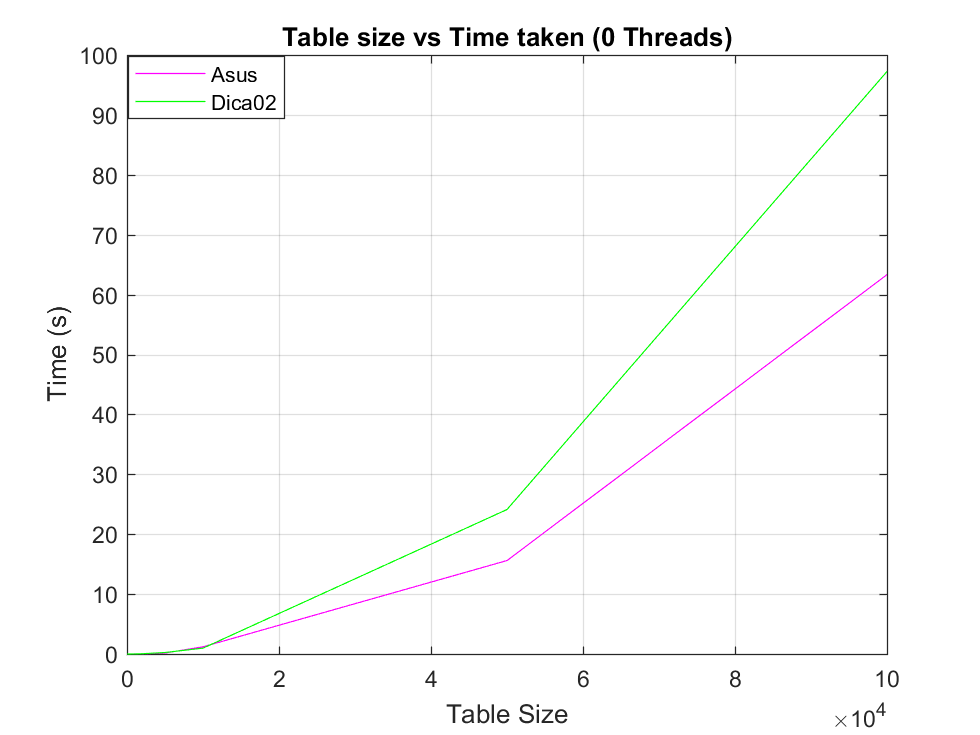
\includegraphics[scale=0.30]{Thread0.png}
\caption{Graph showing the \emph{ASUS} and \emph{Dica02} execution times of the OpenMP algorithm with 0 Threads}
\label{fig: OpenMP Thread0}
\end{figure}
\begin{figure}[h!]
\renewcommand{\thefigure}{\arabic{figure}}
\centering
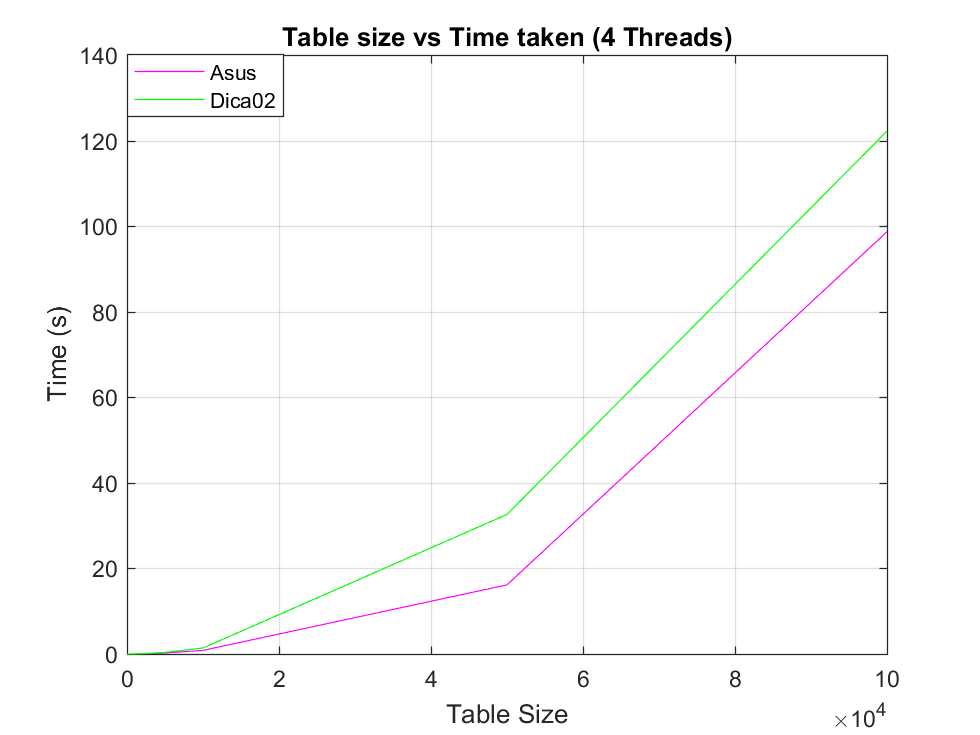
\includegraphics[scale=0.30]{Thread4.png}
\caption{Graph showing the \emph{ASUS} and \emph{Dica02} execution times of the OpenMP algorithm with 4 Threads}
\label{fig: OpenMP Thread4}
\end{figure}
\begin{figure}[h!]
\renewcommand{\thefigure}{\arabic{figure}}
\centering
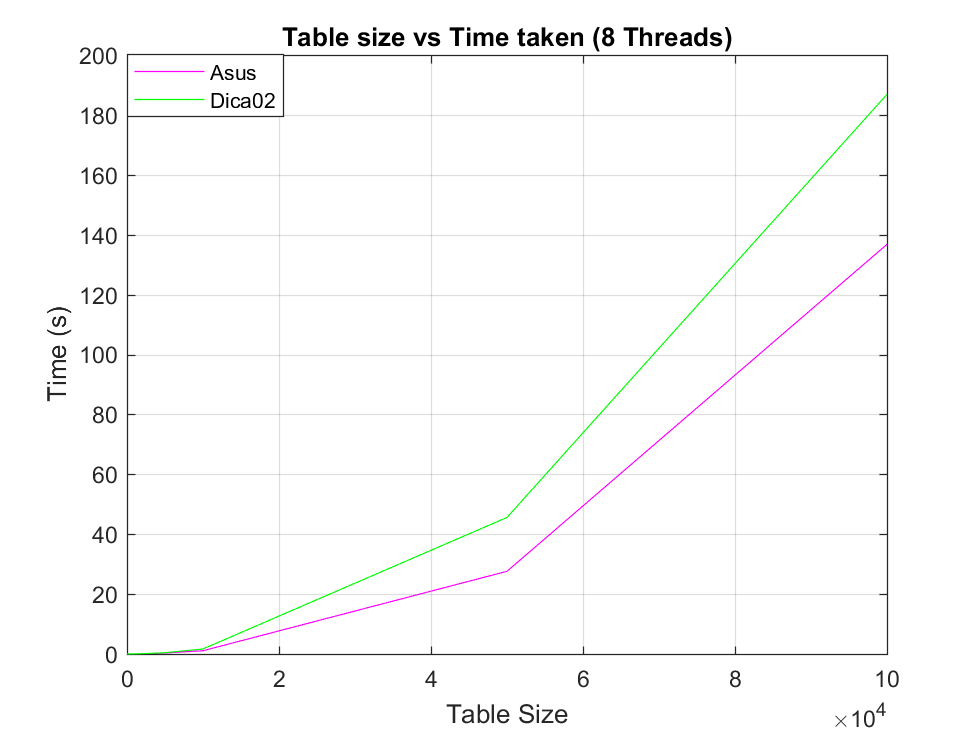
\includegraphics[scale=0.30]{Thread8.png}
\caption{Graph showing the \emph{ASUS} and \emph{Dica02} execution times of the OpenMP algorithm with 8 Threads}
\label{fig: OpenMP Thread8}
\end{figure}
\begin{figure}[h!]
\renewcommand{\thefigure}{\arabic{figure}}
\centering
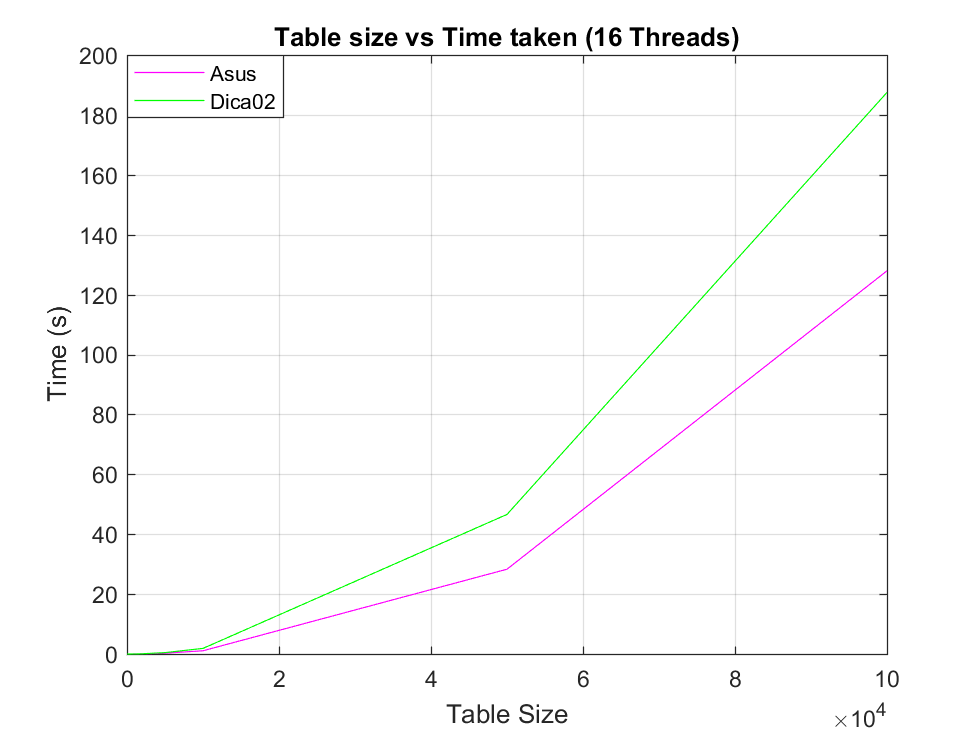
\includegraphics[scale=0.30]{Thread16.png}
\caption{Graph showing the \emph{ASUS} and \emph{Dica02} execution times of the OpenMP algorithm with 16 Threads}
\label{fig: OpenMP Thread16}
\end{figure}
\begin{figure}[h!]
\renewcommand{\thefigure}{\arabic{figure}}
\centering
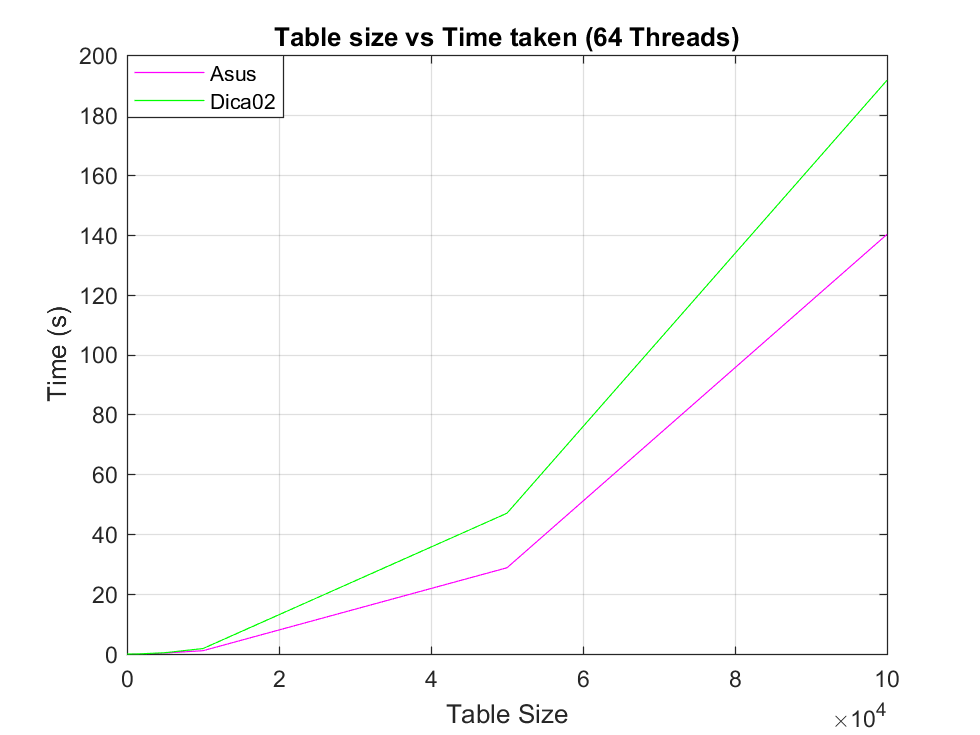
\includegraphics[scale=0.30]{Thread64.png}
\caption{Graph showing the \emph{ASUS} and \emph{Dica02} execution times of the OpenMP algorithm with 64 Threads}
\label{fig: OpenMP Thread64}
\end{figure}
\begin{figure}[h!]
\renewcommand{\thefigure}{\arabic{figure}}
\centering
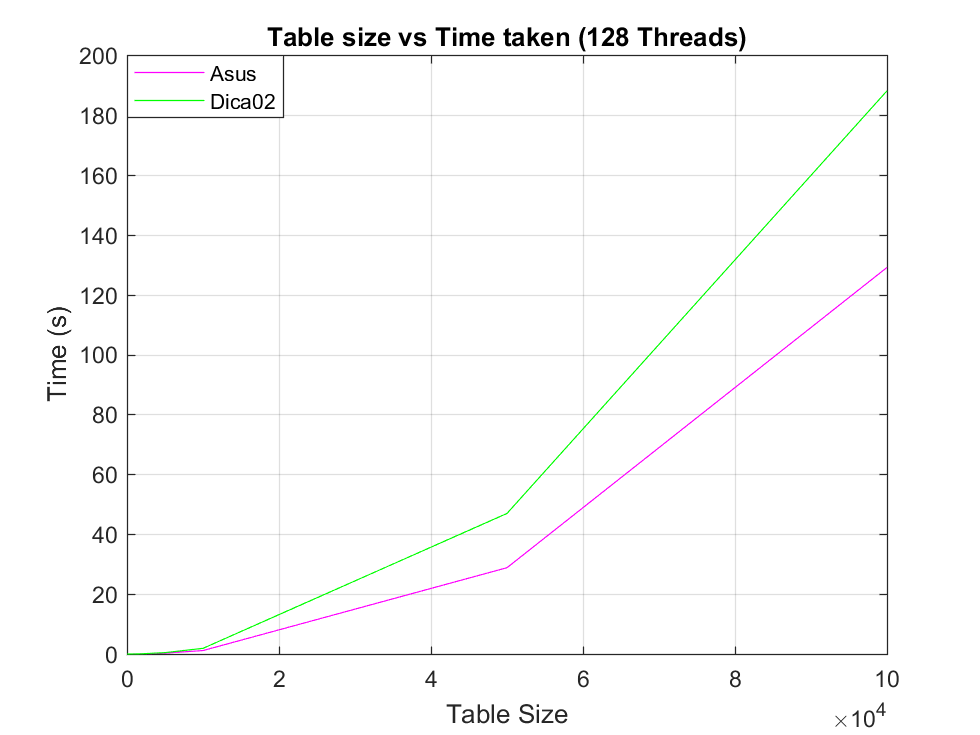
\includegraphics[scale=0.30]{Thread128.png}
\caption{Graph showing the \emph{ASUS} and \emph{Dica02} execution times of the OpenMP algorithm with 128 Threads}
\label{fig: OpenMP Thread128}
\end{figure}

\section{Conclusion}
\label{sec: Conclusion}
The implementation of the two parallel equi-join algorithms of various table sizes (large) have been presented. The criteria defined for success has been met, and the algorithms utilized two programming models, namely MPI and OpenMP. High-level algorithms of each method and model used have been presented and the algorithms were tested on a benchmark device and on the built cluster, and results were presented in various tables and various graphical representations. Due to various time constraint factors, and no prior definition of \emph{large} table size, tables of up to 100000 were generated and tested on as this size could be defined as a large data table set.

\begin{thebibliography}{}

%**************************Intro**************************%
\bibitem{IBM Maintaining}
IBM; \emph{Maintaining Databases}; \url{http://publib.boulder.ibm.com/tividd/td/ITWSA/ITWSA_info45/en_US/HTML/guide/t-expire.html}; Last Accessed: 07/05/2018


%**************************Cluster**************************%
\bibitem{Cluster definition}
Techopedia; \emph{What is Computer Cluster? - Definition from Techopedia}; \url{https://www.techopedia.com/definition/6581/computer-cluster}; Last Accessed: 07/05/2018

\bibitem{RAID}
Rouse, M; \emph{What is disk mirroring (RAID 1)? - Definition from WhatIs.com}; \url{https://searchstorage.techtarget.com/definition/disk-mirroring}; Last Accessed: 07/05/2018

%**************************MPI**************************%
\bibitem{MPI}
Barney, B; \emph{Message Passing Interface (MPI)}; \url{https://computing.llnl.gov/tutorials/mpi/}; Last Accessed: 10/05/2018


%**************************OpenMP**************************%
\bibitem{OpenMP}
Barney, B; \emph{OpenMP}; \url{https://computing.llnl.gov/tutorials/openMP/}; Last Accessed: 10/05/2018



\end{thebibliography}




% that's all folks
\end{document}


